\documentclass[11pt,letterpaper]{article}
\usepackage{naaclhlt2015}
\usepackage{latexsym}

% For citations
\usepackage[authoryear,round]{natbib}
%\usepackage{hyperref}

% For algorithms		
\usepackage{algorithm}
%\usepackage{algorithmic}
\usepackage{algpseudocode}
% \newcommand{\theHalgorithm}{\arabic{algorithm}}


%For figures
\usepackage{graphicx}
\usepackage{subfigure} 
\usepackage{multirow}

\usepackage{amsfonts}
\usepackage{amsmath}
\usepackage{color}
\usepackage{courier}
\usepackage{enumerate}
\usepackage{helvet}
\usepackage{times}
%%%%%%%%%
%% New Commands
%%%%%%%%%

%%%%%%%%%
%% Temporary commands, to be deleted
%%%%%%%%%

\newcommand{\note}[1]{{\tt Note: #1}} % this should be deleted before the submission
\newcommand{\outl}[1]{{\tt Outline: #1}} % this should be deleted before the submission
\newcommand{\notemb}[1]{{\color{blue}MB: #1}}
\newcommand{\noteac}[1]{{\color{cyan}AC: #1}}
\newcommand{\noteme}[1]{{\color{green}ME: #1}}
\newcommand{\fixme}[1]{{{\tt\color{red}[[#1]]}}}
\newcommand{\cut}[1]{}
%%%%%%%%%%%%%%%%%%%%%%%%%%%%%%%%%%%%%%%%%%%%%%%%%%%%%%%
% Command for citation
%\newcommand{\citet}[1]{{\newcite{#1}}}

% Commands for Sections, Figures, Equations, etc.

\newcommand{\secref}[1]{Section~\ref{#1}}
\newcommand{\figref}[1]{Figure~\ref{#1}}
\newcommand{\eqnref}[1]{Equation~\ref{#1}}
\newcommand{\alref}[1]{Algorithm~\ref{#1}}
\newcommand{\tabref}[1]{Table~\ref{#1}}
 
%% Notation

\newcommand{\Ca}{\set{C}}
\newcommand{\Doc}[2]{{D_{#1}^{#2}}}
\newcommand{\dynunc}{\texttt{dynamic-unc}}
\newcommand{\dynconst}{\texttt{dynamic-const}}
\newcommand{\e}[1]{{\mathbb E}\left[ #1 \right]}
\newcommand{\fixkunc}{\texttt{static-k-unc}}
\newcommand{\fixkconst}{\texttt{static-k-const}}
\newcommand{\La}{\set{L}}
\newcommand{\set}[1]{{\mathcal{#1}}}
\newcommand{\Un}{\set{U}}
\newcommand{\vocab}[1]{{\sl #1}}
\newcommand{\Y}{\set{Y}}
\newcommand{\Neu}{\set{N}}
\newcommand{\x}{{\mathbf x}}
\newcommand{\Score}{\mathrm{Score}}
%\newcommand{\N}{\texttt{RND-\-FULL}}
\newcommand{\N}{\texttt{N}}


%% Structured Reading 
\newcommand{\rnd}[1]{\texttt{rnd\_#1}}
\newcommand{\unc}[1]{\texttt{unc\_#1}}
\newcommand{\rndfirst}{\texttt{rnd\_first1}}

\newcommand{\AAL}{\textsc{AAL}}
\newcommand{\SR}{\textsc{structured reading}}


\newcommand{\argmin}{\operatornamewithlimits{argmin}}
\DeclareMathOperator*{\argmax}{arg\,max} 
%\DeclareMathOperator*{\argmin}{arg\,min} 
 
\providecommand{\e}[1]{\ensuremath{\times 10^{#1}}}
\newcommand{\commentout}[1]{}


\newcounter{theexample} \setcounter{theexample}{1}
\newenvironment{example}[1][]{\medskip\noindent {\textbf{Example
\arabic{theexample}. #1} \stepcounter{theexample} \rm}{\medskip}}

\def\sharedaffiliation{%
\end{tabular}
\begin{tabular}{c}}

\setlength\titlebox{6.5cm}    % Expanding the titlebox

\title{Detecting Social Bots on Twitter: An Anytime Active Learning Approach \Thanks{This report was developed as part of a course project for CS579-F14 and is part of the AAL research project at the Machine Learning Lab at IIT.}}

\author{Maria E. Ramirez-Loaiza \\
{\tt mramire8@hawk.iit.edu} \\
Illinois Institute of Technology\\
  	Chicago, IL 60616
}

\date{}

\begin{document}
\maketitle
\begin{abstract}
Abstract here. 
\end{abstract}


% !TEX root = ./master.tex
 
\section{Introduction}

\outl{Active learning}

\outl{Use in social networks}

\outl{tweeter classficiation task}

\outl{challenge}

\outl{proposed method}

\outl{challenges}

\outl{experiments}

\outl{research questions}
	% !TEX root = ./master.tex
 
\section{Methodology}

In this section, we first review standard active learning and then formulate our proposed method. 

\subsection{Problem Formulation}

Let $\La = \{(\x_i, y_i)\}_{i=1}^l$ be a labeled dataset where $\x_i \in
\mathbb{R}^d$ is a $d$-dimensional feature vector that represents a Twitter user timeline and $y_i \in \{y^0=\mathrm{human}, y^1=\mathrm{bot}\}$ is its class label. Let $\Un = \{\x_i\}_{i=l+1}^{m}$ be a set of unlabeled examples. Let $P_\La(y|\x)$ be the conditional probability of $y$ given $\x$ according to a classifier trained on $\La$.

Typical pool-based active learning selects instances $\Un^* \subseteq \Un$ to
be labeled by a human annotator ({\it oracle}) and appended to $\La$. Assuming
a prespecified annotation budget $B$ and an annotation cost function $C(\x)$,
the goal of the active learning algorithm ({\it student}) is to select $\Un^*$
to minimize the classifier's generalization error subject to the budget
constraints:
%
\begin{multline}
\label{eq.pool}
\Un^* \leftarrow \argmin_{\Un_i \subseteq \Un} Err(P_{\La\ \cup\ \Un_i}(y|\x)) \\
\hbox{ s.t. } \sum_{\x_j\in \Un_i} C(\x_j) \le B
\end{multline}

Equation~\ref{eq.pool} is typically optimized by greedy algorithms, selecting
one or more examples at a time according to some heuristic criterion that
estimates the utility of each labeled example. A common approach is to request
a label for the unlabeled instance that maximizes benefit-cost 
ratio: $\x_i^* \leftarrow \argmax_{\x_i \in \Un} \frac{U(\x_i)}{C(\x_i)}$.

Various definitions of utility $U(\cdot)$ are used in the literature, such as
expected error reduction~\cite{roy:icml01} and classifier
uncertainty~\cite{lewis:sigir94}.  In this paper, we use uncertainty sampling for our formulation. More formally, uncertainty sampling queries the instances whose predicted posterior probability is the least confident, redefining \eqnref{eq.pool}: 

\begin{equation}\label{eq:unc}
 \x^* \leftarrow \argmax_{\x_i \in \Un} \left(1- \max_{y \in Y} P_{\La}(\hat{y}|\x_i) \right)	
\end{equation}

\eqnref{eq:unc} uses conditional error as a measure of confidence.

%\cut{ Another common definition of uncertainty is entropy as the utility measure \cite{shannon:bstj48}:
%
%\begin{equation}\label{eq:ent}
% \x^* \leftarrow \argmax_{\x_i \in \Un} \left( - \sum_{y \in Y} P_{\La}(\hat{y}|\x_i) \log(P_{\La}(\hat{y}|\x_i))      \right)	
%\end{equation}
%}
We propose the use of an anytime active learning technique to save annotation cost by controlling what the oracle sees \citep{ramirez:aaai14}. The idea is that the student selects the most representative tweet of a user timeline and queries the oracle for the label. We define an alternative formulation of the active learning problem in which the student has the added capability of presenting one tweet the human oracle to request a label. 

Let $s_i^k$ be the $k$-th tweet in user $\x_i$ timeline. Each tweet is scored by a function $TS(\cdot)$ which determines how important is a tweet for labeling. We build upon \eqnref{eq:unc} and incorporate the tweet selection into the student's objective:
%
\begin{multline} \label{eq:obj}
    \argmax_{ \x_i \in \Un} 1- \max_{y \in Y} P_{\La}(\hat{y}|\x_i) \times max_{s_i^k \in \x_i} TS(s_i^k)
\end{multline}
%
In our experiments, we define $TS(\cdot)$ as the tweet most likely to be labeled. Intuitively, we want to select a tweet that allows the oracle to determine if the author of the tweet is human or not. Also, we want that tweet to be likely to be labeled since we optimize the budget simultaneously. Formally, we define the function as: 
%
\begin{align}
	TS(s_i^k) = \max_{y} T(y_i | s_i^k)
\end{align}
%
\noindent
where $T(\cdot)$  is a tweet probabilistic classifier that determines how likely is an individual tweet to be bot or human generated. In practice, we use tweets $s_i^k \in \x_i \in \La$ to train the tweet classifier.  

%%==============================================================

\section{Experimental Evaluation}

\subsection{Data Collection}
%
Our experiments uses data collected from Twitter based on the \textbf{Social Honeypots} dataset \cite{lee:aaai11}. We use a subset of a collection of known legitimate and bot account user names, to build our own dataset. We collected the most recent timeline of each user up to 200 tweets. We collected 883 legitimate user and 898 bot accounts. 

The data was further filtered by removing accounts whose last activity was older than 2014, eliminating 45 and 173 accounts from legitimate and bots respectively. For our active learning experiments, we report average of five trials on a train-test split. 


\subsection{Data Preprocessing}
%
Each tweet was tokenized by words, ignoring punctuation, collapsing URLs and mentions. Every token was converted to lower case and stemmed using a Porter stemmer. The resulting tokens were used to form a TF-IDF feature vector using unigrams. To reduce the size of the dictionary terms that appear less than five times are removed. The final dictionary size is of 13399 features. \tabref{tab:data} characteristics of the representation.

\begin{table}[htdp]
\caption{Collected data from Twitter per type of user}
\begin{center}
\begin{tabular}{|c|c|c|c|} \hline
\textbf{Class} & \textbf{N. Users} &\textbf{Avg. Tweets} \\  \hline
Human & 838 & 199 \\ \hline
Bots & 725  & 196 \\ \hline
\end{tabular}
\end{center}
\label{tab:data}
\end{table}%
 
\subsection{Simulations}

\textbf{Simulated Oracle.} We simulated the oracle by training a logistic regression classifier with L2 regularization, with the default regularization C=1 parameter. The classifier was trained on the tweets in the train-split of the data. At every iteration the simulated oracle will return the predicted label of the queried tweet. 

\textbf{Student}. For the student, we use a logistic regression classifier with the same configuration of the simulated oracle. We start every experiment with a small amount of labeled data, 50 user's timeline. $T$ classifier is bootstrapped with the individual tweets of the initial 50 users. 

%\input{expeval}
% !TEX root = ./master.tex
 
\section{Results and Discussion}

\subsection{Classification Methods }
We tested several probabilistic classifiers and analyzed the learning curve by randomly sampling. \figref{fig:class} show the accuracy learning curve of logistic regress with L1 and C=1, i.e., {\tt{lr-l1-c1}}, L2 regularization with C=1, and C=10, i.e., {\tt{lr-l2-c1}} and {\tt{lr-l2-c10}}, and multinomial naive babes, i.e., {\tt{mnb}}. We observe that {\tt{mnb}} has the best performance followed by {\tt{lr-l2}} with c=1 and c=10. 

\begin{figure*}[t]
	%\vskip -0.2in
	%\begin{center}
	\centering
		\centerline{
%			\subfigure[IMDB ]{
				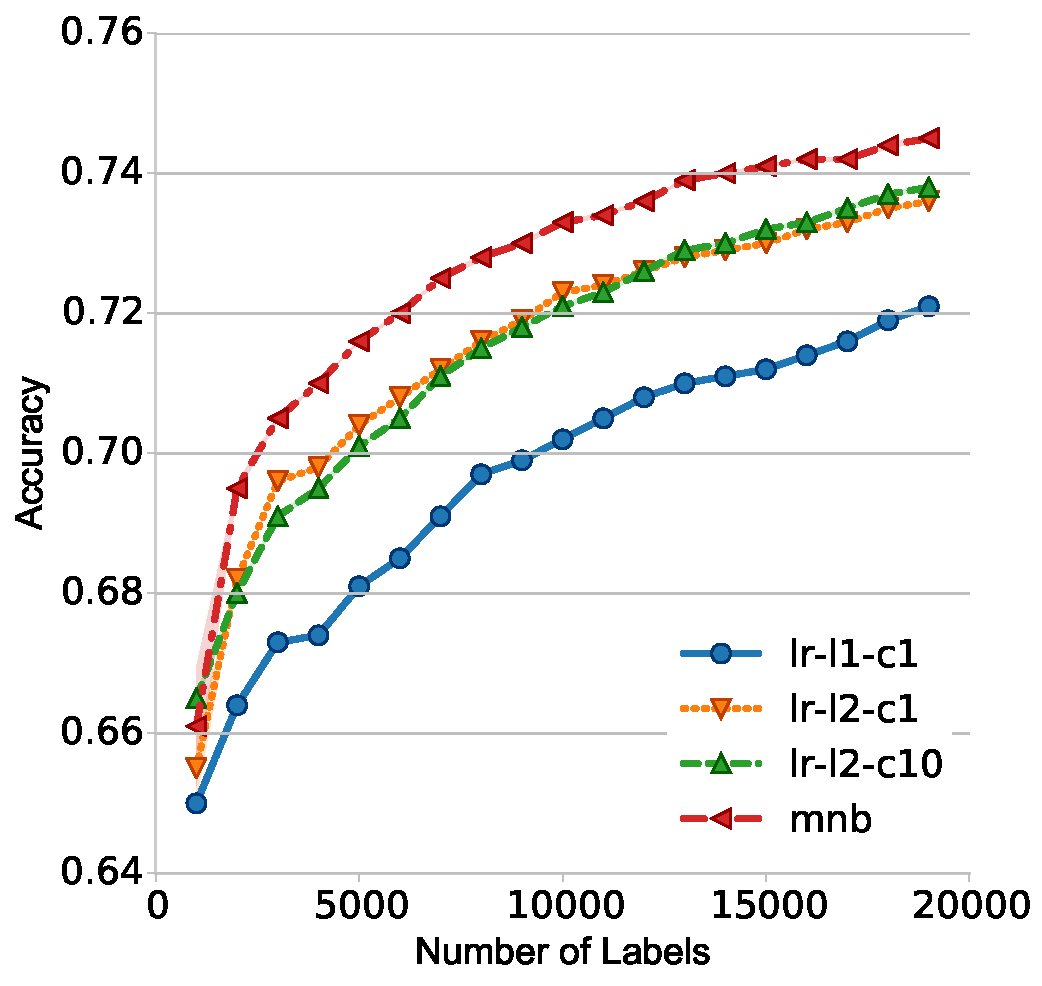
\includegraphics[width=0.9\columnwidth]{fig/models-accu.pdf}
			\label{fig:class}	
%			}	
		}
		\vskip -0.15in
		\caption{Classification models induced on tweets. The performance of four probabilistic classifiers on tweeter data. The budget is the number of labels.}
		\label{fig:user}
	%\end{center}
	\vskip -0.1in
\end{figure*}

\subsection{Data Representation}

We set to find an appropriate data feature vector representation. We tested three data processing options: lower case, URL and mention collapse. We tried all eight combinations and tested using a five fold cross validation. In average, the accuracy of the classifier is 82.5\% ($+/-$ 0.4). We observed that there are no significant differences among all variations, we use the combination of all options active to reduce the size of the dictionary. 

%\subsection{Classification of Individual Tweets}
%\begin{figure*}[t]
%	%\vskip -0.2in
%	%\begin{center}
%	\centering
%		\centerline{
%			\subfigure[IMDB ]{
%				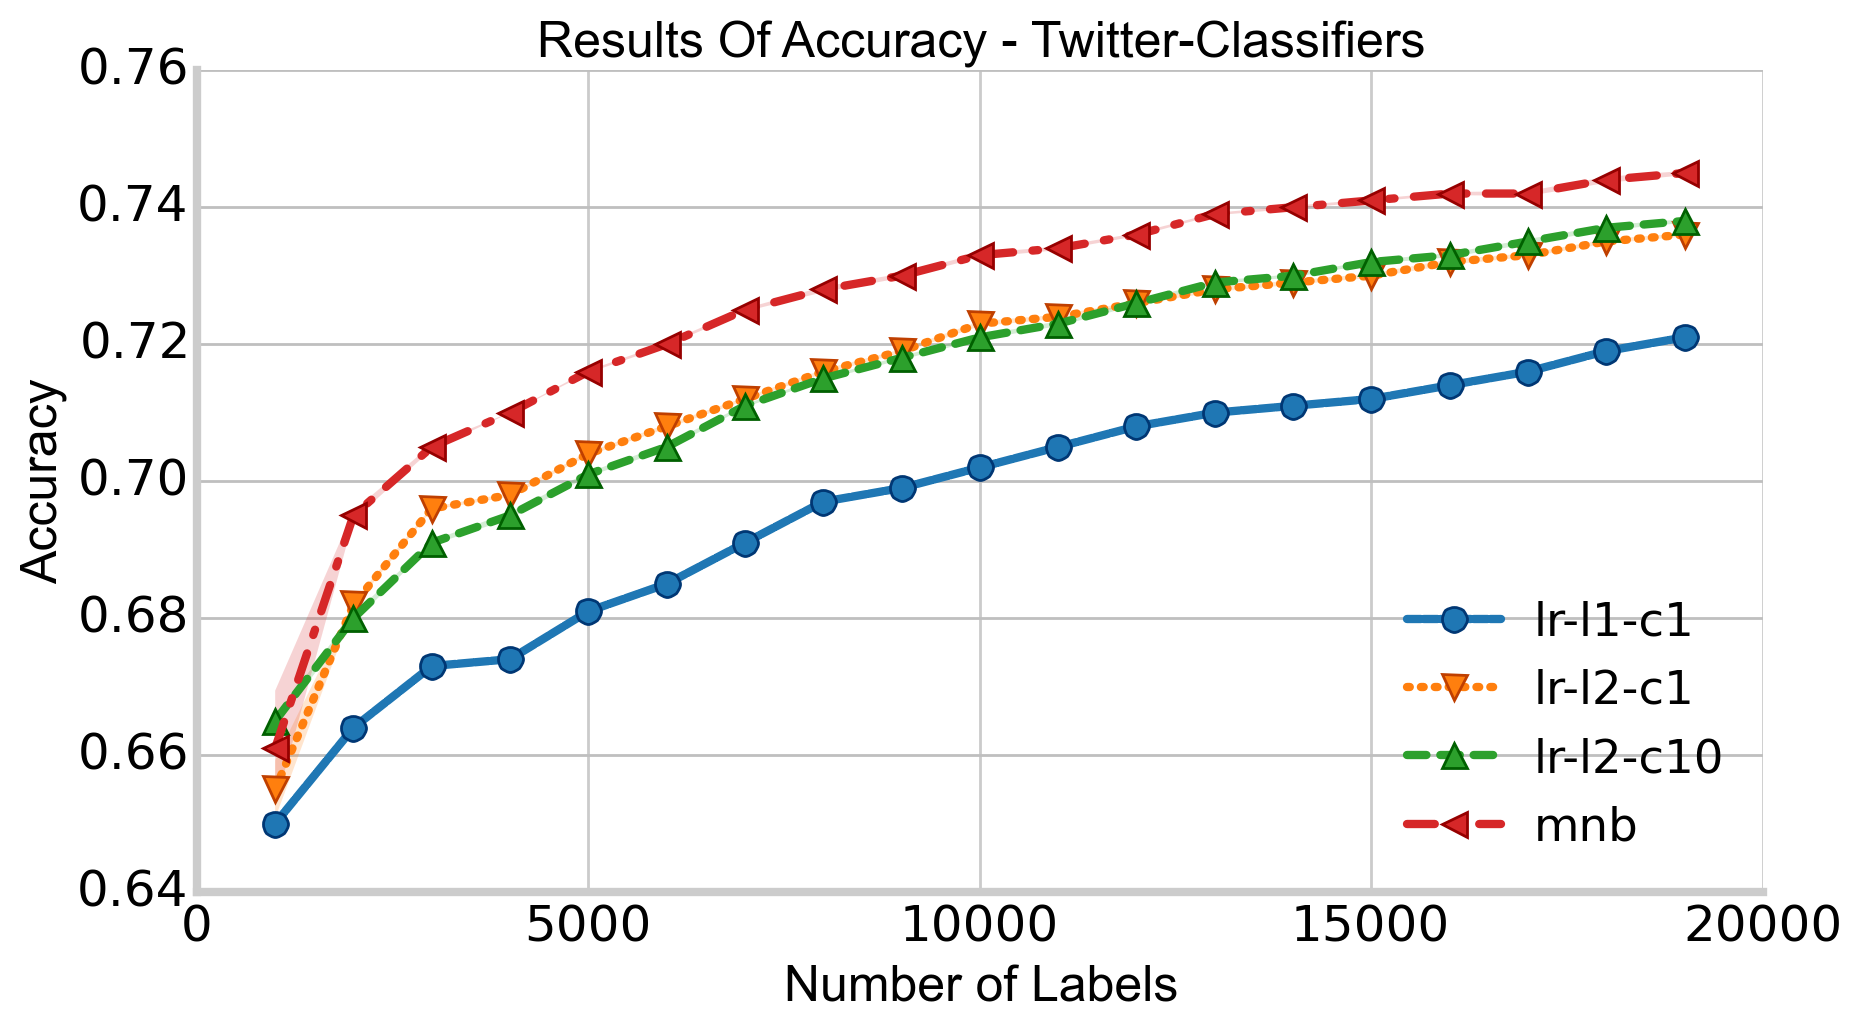
\includegraphics[width=0.7\columnwidth]{fig/twitter-classifiersaccuracy.png}
%			\label{fig:class}	
%			}	
%		}
%		\vskip -0.15in
%		\caption{Classification models induced on tweets.}
%		\label{fig:user}
%	%\end{center}
%	\vskip -0.1in
%\end{figure*}
%
%\begin{figure*}[t]
%	%\vskip -0.2in
%	%\begin{center}
%	\centering
%			\subfigure[IMDB ]{
%				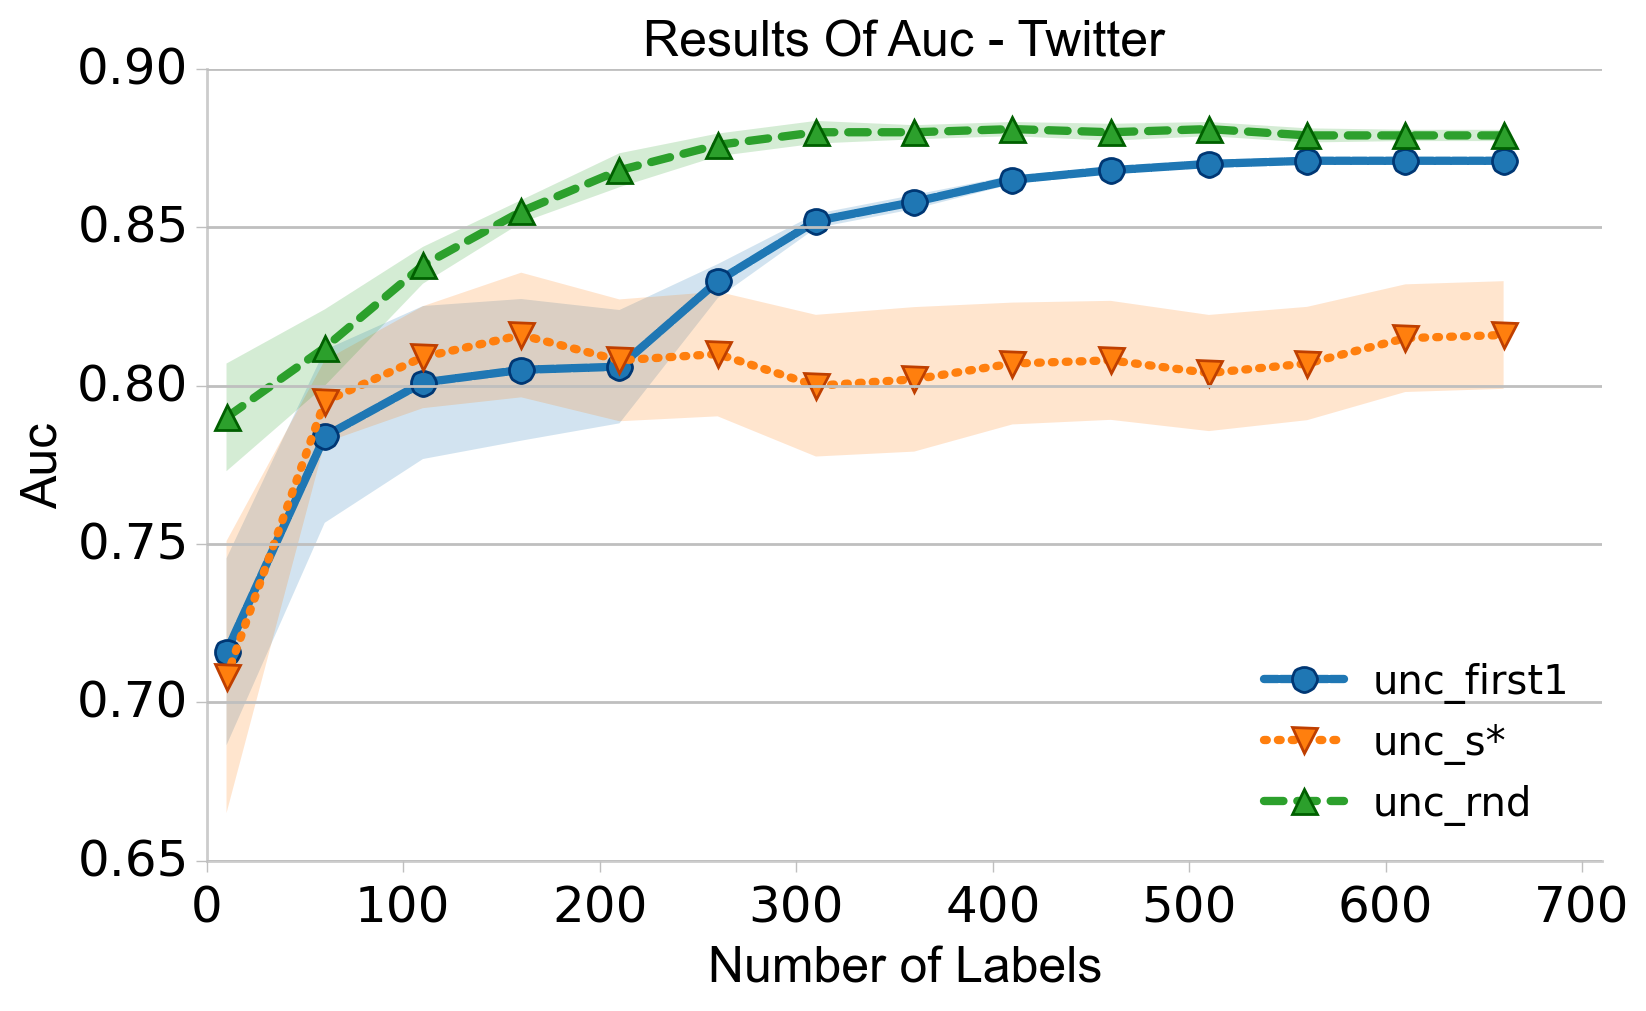
\includegraphics[width=0.7\columnwidth]{fig/twitterauc.png}
%			\label{fig:class}	
%			}	
%		\vskip -0.15in
%		\caption{Active Learning.}
%		\label{fig:user}
%	%\end{center}
%	\vskip -0.1in
%\end{figure*}

\subsection{Other Features}
We tested the use of other features derived from the text such uniqueness of the terms. For example, a bot may use the same terms over and over thus the number unique terms will be low. The uniqueness formulations was: 
%
\begin{equation}
Unique(\x_i) = \frac{TF}{UniqueTerms}
\end{equation}
%
\noindent where $TF$ is the term frequency. We tested this feature representation and obtained 54\% accuracy (+/-0.0). We conjecture that the difference of this measure between the two classes is not significant to have enough classification power. 

\subsection{Error Analysis}
We analyzed a fully trained classifier and reviewed the mistakes made on a test split. The idea is to identify if the classifier is able to reasonable annotate individual tweets, from a human point of view. We used a {\tt{lr-l2-c1}} and we verify the incorrect labels with high incorrect probability. We found that the classifier usually mislabels tweets in other languages other than english, due to low number of examples. Common mistakes, also occurred on tweets with only mentions and URLs. \tabref{tab:twmistakes} show examples of mistakes made by the classifier. 

\begin{table*}[htdp]
\begin{center}
\begin{tabular}{|p{5cm}|c|l|}
\hline \textbf{Tweet Example} & \textbf{True Label} & \textbf{Observation} \\ \hline
THIS\_IS\_A\_MENTION THIS\_IS\_A\_MENTION  otro ,\textbf{que} a lo mejor no sabe que es la udef & Bot & Other languages \\ \hline
THIS\_IS\_A\_MENTION ?effective \textbf{sales} and \textbf{marketing} is getting to the truth as quickly as possible? \#sales \#marketing \#cmworl   & Human & Terms used \\ \hline
rt THIS\_IS\_A\_MENTION \#goroyals  & Bot & Only mention \\ \hline
\end{tabular}
\caption{Example tweets incorrectly labeled by a {\tt{lr-l2l-c1}} classifier. The terms in bold face correspond to the highest weight value according to the classifier.  }
\end{center}
\label{tab:twmistakes}
\end{table*}%
 

\subsection{Active Learning Experiments}
We tested several method of active learning where the learner algorithm picks a tweet from the timeline of a user and requests the label. We tried several approaches as follows:
\begin{description}
\item[\unc{first1}] is a joint formulation of uncertainty of the timeline and maximum first tweet approach. This is a baseline. 
\item[\unc{rnd}] is a joint formulation of uncertainty  of the timeline and a random tweet. This is a baseline
\item[\unc{sr}] is a joint formulation of uncertainty and the best tweet. We tested using a logistic regression model and a multinomial naive bayes model. 
\end{description}

\figref{fig:sr} shows the results accuracy results of the tested models. We observe that the multinomial naive bayes approach has the worst performance. \unc{first1} and \unc{rnd} are the close in performance, however, selecting random tweets perform slightly better in early iterations. We argue that the oracle responses are imbalanced thus introducing noise in the training data. \tabref{tab:cm-ora} shows the confusion matrix of the oracle after labeling 690 tweets selected by the learning algorithm. Note that \unc{first1} and \unc{rnd} have a balanced percentage of error for both human and bot labels, whereas \unc{sr} mistakenly classifies more tweets as bots. 

\begin{figure*}[t]
	%\vskip -0.2in
	%\begin{center}
	\centering
%			\subfigure[IMDB ]{
				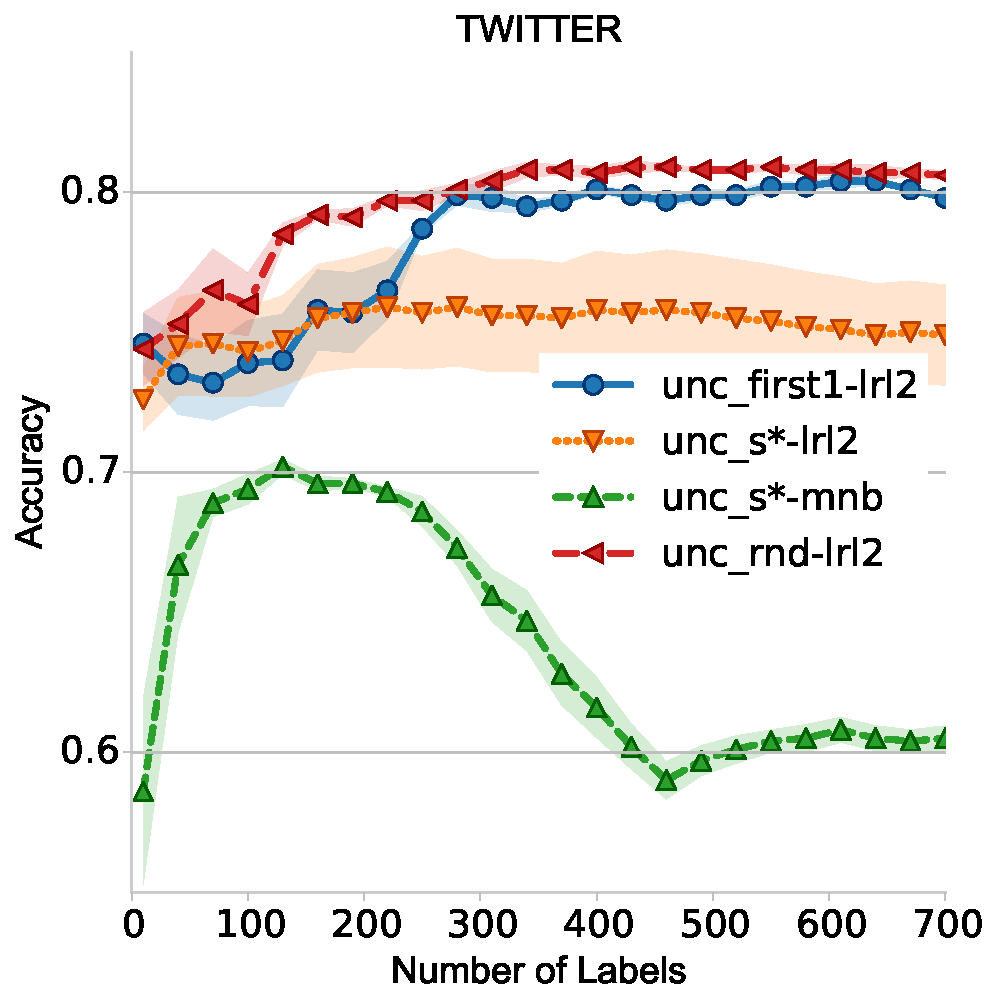
\includegraphics[width=0.9\columnwidth]{fig/sr-accuracy.pdf}
			\label{fig:class}	
%			}	
		\vskip -0.15in
		\caption{Active learning experiments. Results averaged over five trial.}
		\label{fig:sr}
	%\end{center}
	\vskip -0.1in
\end{figure*}

\begin{table*}[!ht]
	%\vskip -0.2in
	\begin{small}
	\begin{center}
		\centering{
			\begin{tabular}{|c|c|c|c|} 
				\multicolumn{4}{c}{\textbf{\unc{first1}-lr}} \\
				\hline \textbf{T. Size }  & & \textbf{H} & \textbf{B} \\ \hline
				690 	&\textbf{H	}	& 40 	& 12 \\ \cline{2-4}
				 	& \textbf{B	}	&12 	& 36 \\ \hline
			\end{tabular} \quad
			\begin{tabular}{|c|c|c|c|} 
				\multicolumn{4}{c}{\textbf{\unc{sr}-lr}} \\
				 \hline \textbf{T. Size }  & & \textbf{H} & \textbf{B} \\ \hline
				690 	&\textbf{ H}	& 35 	& 19 \\ \cline{2-4}
				 	&\textbf{ B	}& 8 	& 39 \\ \hline
			\end{tabular} \quad
			\begin{tabular}{|c|c|c|c|} 
				\multicolumn{4}{c}{\textbf{\unc{sr}-mnb}} \\
				 \hline \textbf{T. Size }  & & \textbf{H} & \textbf{B} \\ \hline
				690 	& \textbf{H}	& 31 	& 23 \\ \cline{2-4}
				 	& \textbf{B}	& 8 	&38 \\ \hline
			\end{tabular}
			\begin{tabular}{|c|c|c|c|} 
				\multicolumn{4}{c}{\textbf{\unc{rnd}}} \\
				 \hline \textbf{T. Size }  & & \textbf{H} & \textbf{B} \\ \hline
				690 	& \textbf{H}	& 40 	& 10 \\ \cline{2-4}
				 	& \textbf{B}	& 11 	& 39 \\ \hline
			\end{tabular}
			}
			\caption{Oracle confusion matrix for different calibration methods on the Twitter dataset. The matrix is given in percentage with respected to the training size (\textbf{T.Size}). \textbf{H} are human labels and \textbf{B} are bot labels. Each row are true labels and columns are predicted by the classifier. }
		\label{tab:cm-ora}
		\vskip -0.25in
	\end{center}
	\end{small}
\end{table*}


\subsection{Other models and Bootstrap Effect}

An important element of the active learning strategy is the bootstrap size of the training data. Bootstrap size can affect how good are the decision of the learner at early iterations. We tested sizes $bt \in \{10, 50, 100\}$ using \SR\ approaches and a logistic regression with L2 regularizations. \figref{fig:bt} shows the learning curve of the methods with different bootstrap sizes. We observe that the differences are not significant (note the standard error per method, i.e., shadowed in the graph), however, the smallest bootstrap is worse than using 100 user timelines. 

\begin{figure*}[t]
	\centering{
			\subfigure[Bootstrap Effect ]{
				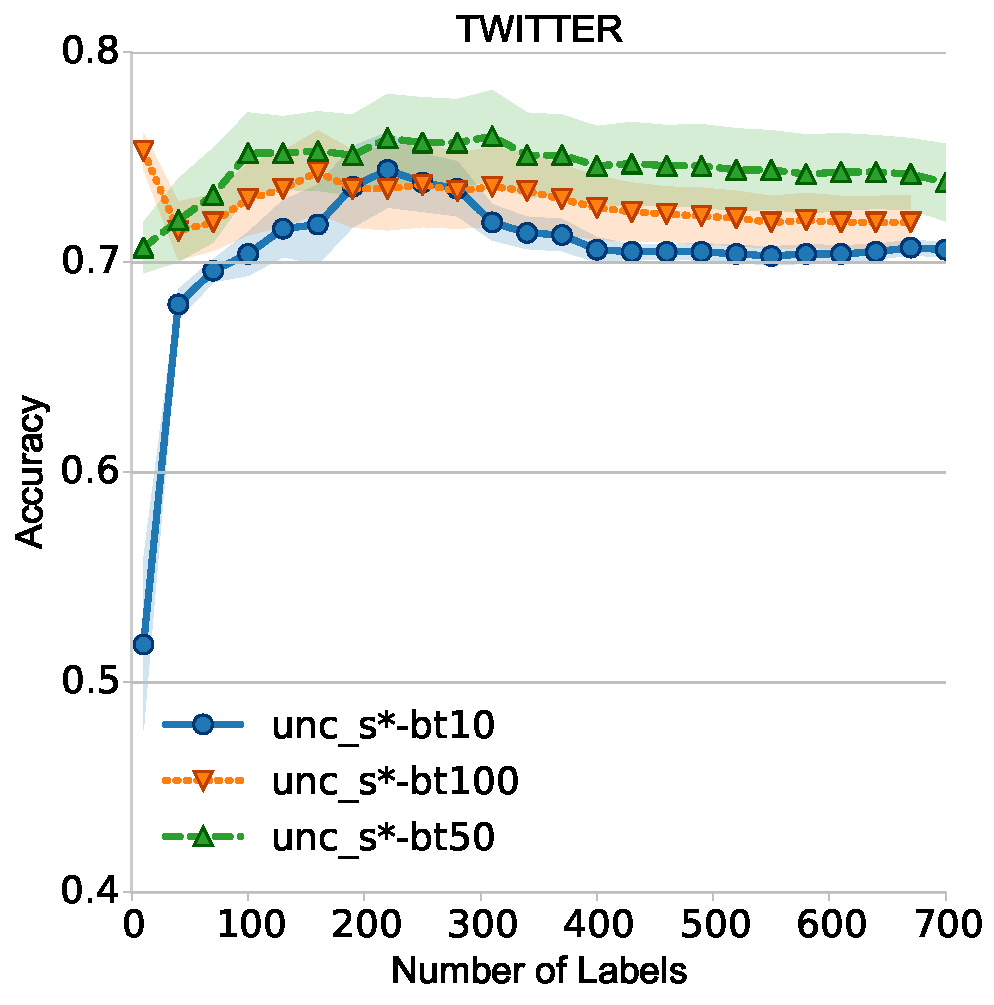
\includegraphics[width=0.8\columnwidth]{fig/bt-accuracy-twitter.pdf}
			\label{fig:bt}	
			} \quad		
			\subfigure[Adaptive Penalty ]{
				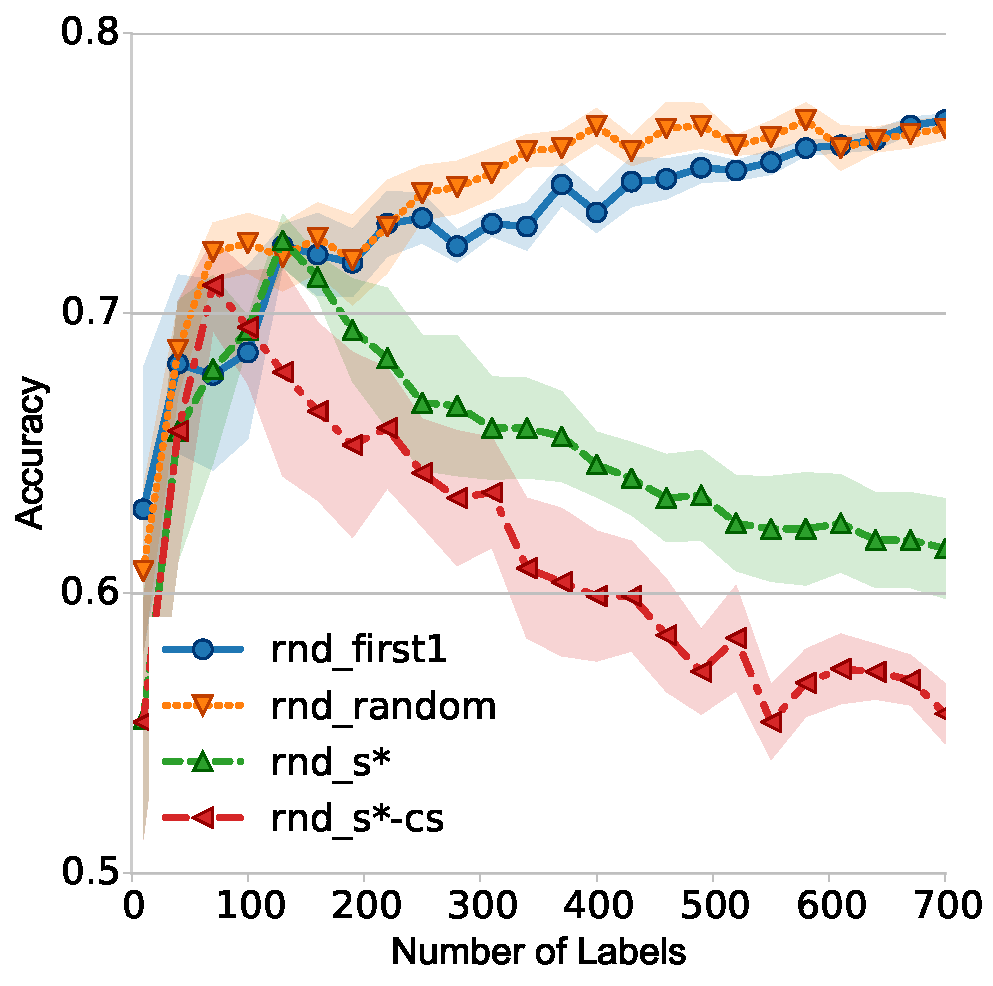
\includegraphics[width=0.8\columnwidth]{fig/lradapt-accuracy-twitter.pdf}
			\label{fig:penalty}	
			}	
		}
		\vskip -0.15in
		\caption{Effect of penalty and bootstrap on the \SR\ methods}
	\vskip -0.1in
\end{figure*}

We also wanted to test if a fixed penalty for the logistic regression model can improve the performance of our proposed method. \figref{fig:penalty} shows the effect of changing the penalty of the model as the training data also changes. We used a random sampling method to isolate the effect of the penalty on the tweet selecting. We observed that the effect of the change does not improve the \SR\ methods to be comparable with the random and first1 baseline. 
% !TEX root = ./master.tex
 
\section{Related Work}

The current work on social bot detection typically uses network analysis techniques to construct complex features and induce a probabilistic classifier. \cite{} proposed a classifier trained on \fixme{list the features}

\noteme{add more related work}

The described methods on previous studies rely on available datasets, which are expensive to build. To the best of our knowledge, our work is the first attempt to use active learning to build a social bot classifier. Furthermore, it is the first attempt to use an anytime active learning approach to address the task. 
% !TEX root = ./master.tex
 
\section{Conclusions}

We proposed an active learning method to detect bot operated twitter accounts using a tweet from the users timeline. Identifying the automated nature of an account is a hard problem. We discuss possible alternative to address the tweet selection method. 



\bibliographystyle{plainnat}
\bibliography{bib/abr,bib/bib} 

\end{document}
